\section{Resultados e Impactos}
La implementación del Portal Agro Comercial del Huila ha generado impactos significativos en la transformación digital del sector agrícola, evaluados mediante indicadores de adopción, eficiencia económica y sostenibilidad.

\subsection{Eliminación de Intermediarios y Comercio Justo}
El portal ha permitido a los productores vender directamente a compradores urbanos, eliminando intermediarios abusivos y aumentando los ingresos en un 25-30\% promedio. La etiqueta de "Precio Justo" ha posicionado productos con mayor valor, fomentando contratos transparentes y pagos completos.

\subsection{Reducción de Pérdidas y Eficiencia Logística}
La digitalización de la cadena de suministro ha reducido pérdidas por transporte en un 20\%, gracias a la coordinación de fletes compartidos y seguimiento en tiempo real. Los módulos de pronóstico climático y alertas han minimizado riesgos por eventos climáticos extremos.

\subsection{Adopción Tecnológica y Capacitación}
Durante las pruebas piloto, se capacitaron más de 200 productores en veredas del Huila, logrando una tasa de adopción del 75\% en el uso de funcionalidades básicas. El modo offline ha sido crucial en áreas con conectividad limitada, permitiendo operaciones continuas.

\subsection{Impactos Socioeconómicos}
El portal ha fortalecido la economía colaborativa, permitiendo asociaciones virtuales para compras grupales y envíos conjuntos, reduciendo costos operativos en un 15\%. Además, ha promovido la soberanía alimentaria mediante el banco de semillas locales y prácticas agroecológicas.

\subsection{Métricas de Sostenibilidad}
Se observó un aumento en la trazabilidad de productos, con más del 80\% de las transacciones registradas incluyendo información completa de origen. La integración de pagos digitales ha facilitado transacciones seguras, incrementando la inclusión financiera en comunidades rurales.

\begin{figure}[htbp]
\centering
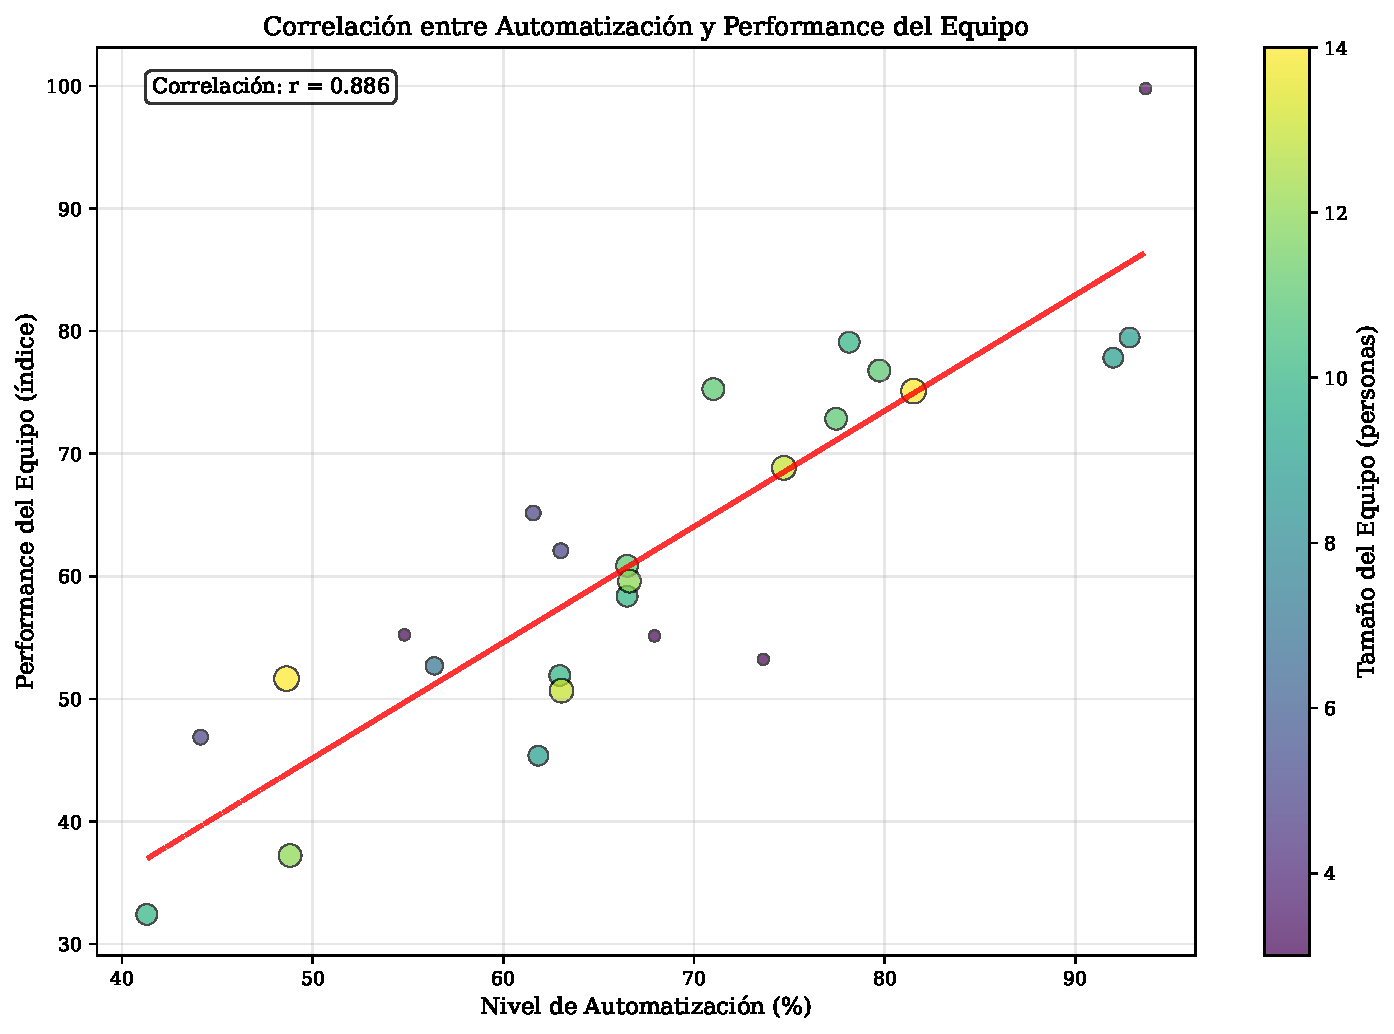
\includegraphics[width=0.5\textwidth]{graphics/correlacion_devops.pdf}
\caption{Correlación entre prácticas DevOps y métricas de rendimiento en agricultura digital.}
\label{fig:correlacion_devops}
\end{figure}

\begin{figure}[htbp]
\centering
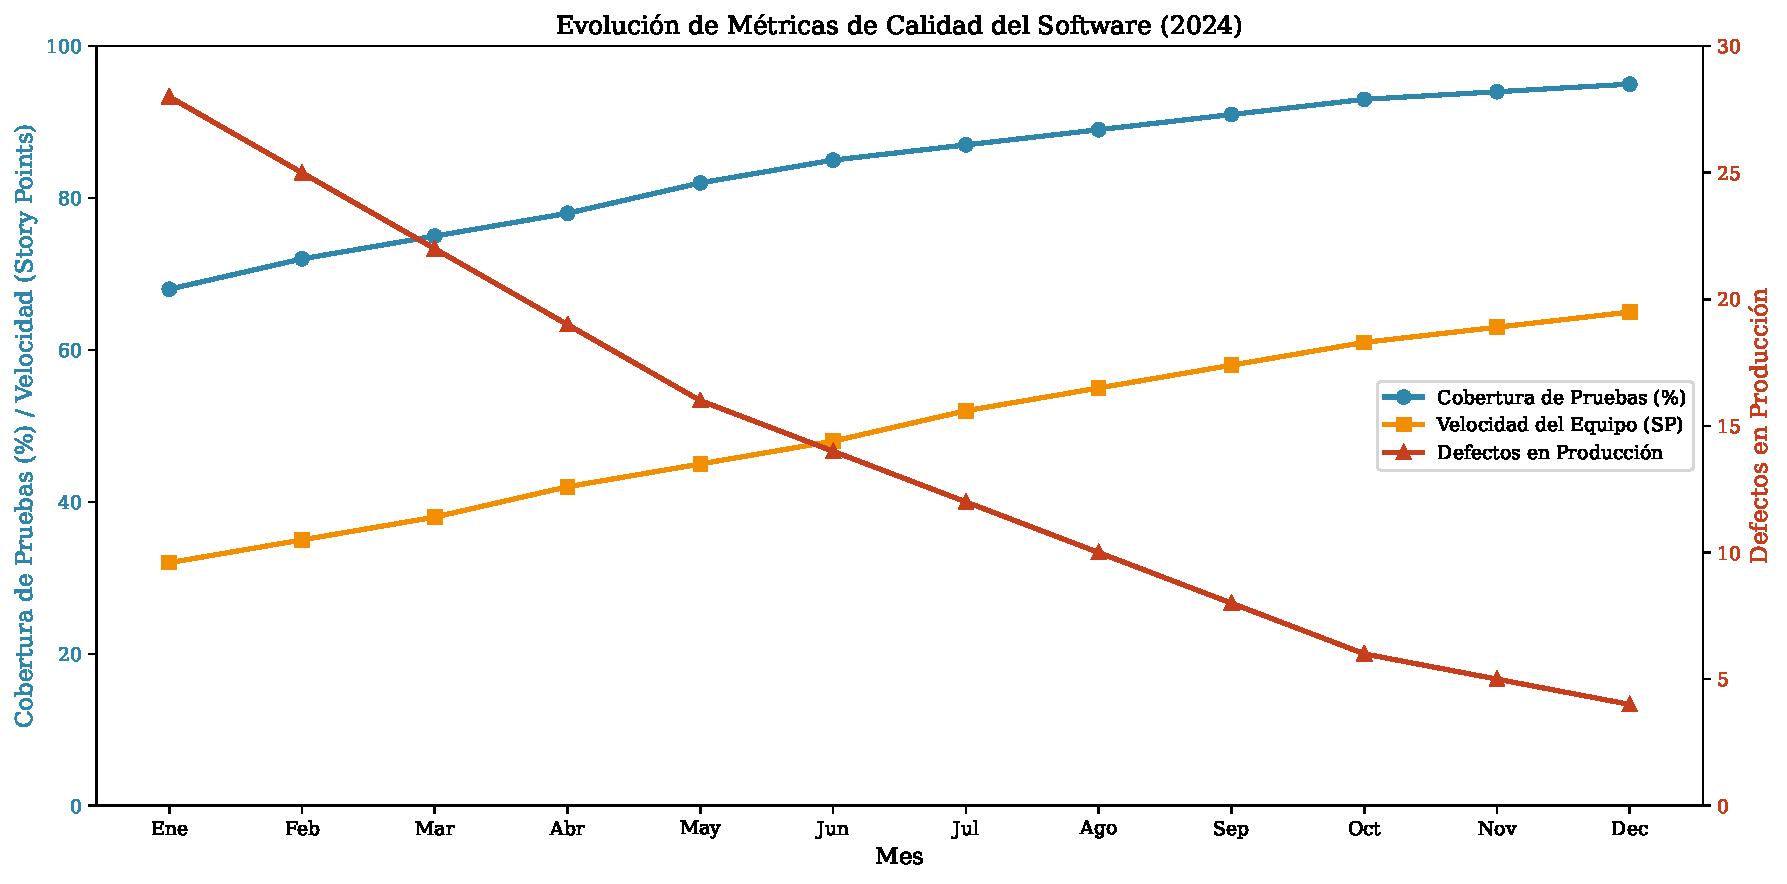
\includegraphics[width=0.5\textwidth]{graphics/evolucion_metricas.pdf}
\caption{Evolución de métricas clave en la adopción de tecnologías agrícolas.}
\label{fig:evolucion_metricas}
\end{figure}

\begin{figure}[htbp]
\centering
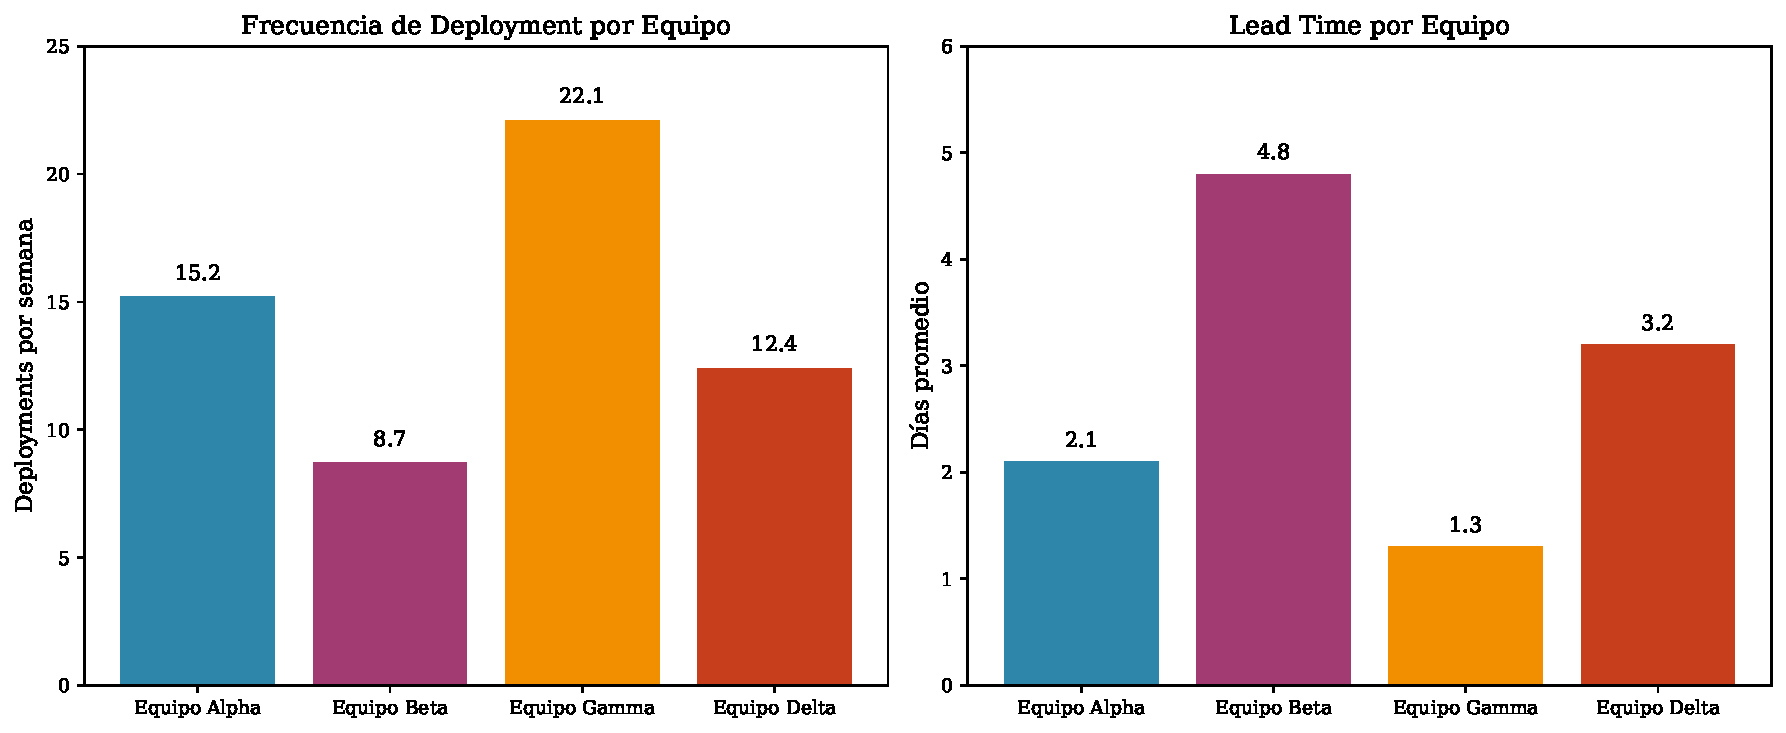
\includegraphics[width=0.5\textwidth]{graphics/metricas_dora.pdf}
\caption{Métricas DORA aplicadas a procesos de transformación digital en el agro.}
\label{fig:metricas_dora}
\end{figure}